% https://tex.stackexchange.com/questions/157222/putting-figures-side-by-side-using-minipage
\documentclass{article}

\usepackage{tikz}
\usetikzlibrary{lindenmayersystems}

\tikzset{
  % https://github.com/pgf-tikz/pgf/blob/master/doc/generic/pgf/text-en/pgfmanual-en-library-lsystems.tex
  Koch curve/.style = {
    l-system={
      rule set={F -> F-F++F-F}, % state transition
      axiom=F++F++F, % initial state, triangle
      step=1pt,
      angle=60,
      #1
    }
  }
}

\begin{document}
    ok, this is going on and on

    \noindent
    \begin{minipage}{.32\textwidth}
    \centering
    \begin{tikzpicture}
    \draw[Koch curve={order=0,step=100pt}] l-system -- cycle;
    \end{tikzpicture}
    \end{minipage}%
    \begin{minipage}{.32\textwidth}
    \centering
    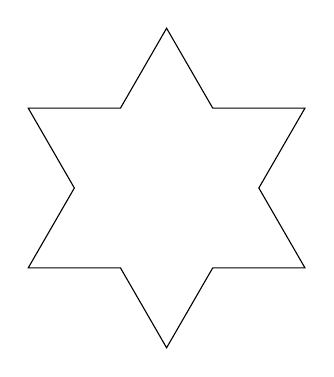
\begin{tikzpicture}
    \draw[Koch curve={order=1,step=100pt/3}] l-system -- cycle;
    \end{tikzpicture}
    \end{minipage}%
    \begin{minipage}{.32\textwidth}
    \centering
    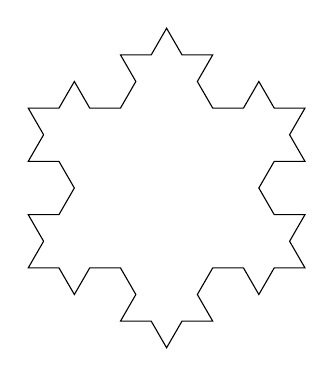
\begin{tikzpicture}
    \draw[Koch curve={order=2,step=100pt/(3^2)}] l-system -- cycle;
    \end{tikzpicture}
    \end{minipage}%
    \begin{minipage}{.32\textwidth}
    \centering
    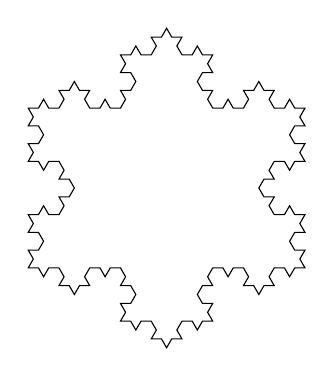
\begin{tikzpicture}
    \draw[Koch curve={order=3,step=100pt/(3^3)}] l-system -- cycle;
    \end{tikzpicture}
    \end{minipage}%


\end{document}
